% Offizielle Beispieldatei für beamer-Vorlage aus tubslatex Version 0.3beta2
\documentclass[fleqn,11pt,aspectratio=43,table]{beamer}
\usepackage[ngerman]{babel}
\usepackage[utf8x]{inputenc}
\usepackage{graphicx}
\usepackage{caption}
\usepackage{subcaption}
\usetheme[%
yellow,                  % secondary color (yellow/orange/blue/green/violet)
light,                  % brightness (light,medium,dark)
tocinheader,           % toc in header
%nosubsectionsinheader, % no subsections in header toc
nexus,                 % corporate design font
lnum,                  % NOTE: only available since tubslatex 1.01,
% use "Versalziffern" instead of "Mediaevalziffern"
]{tubs}

% Titelseite
\title{SecureBlue++}
\subtitle{Seminar Informatik WS 2016/2017 Verteilte Systeme:\\Secure Trusted Execution for Resilient Distributed Systems}
\author{Stephan Mielke}
\date{14. Dezember 2016}
% Titelgrafik, automatisch beschnitten, Weitere Optionen: <scaled/cropx/cropy>
\titlegraphic[cropped]{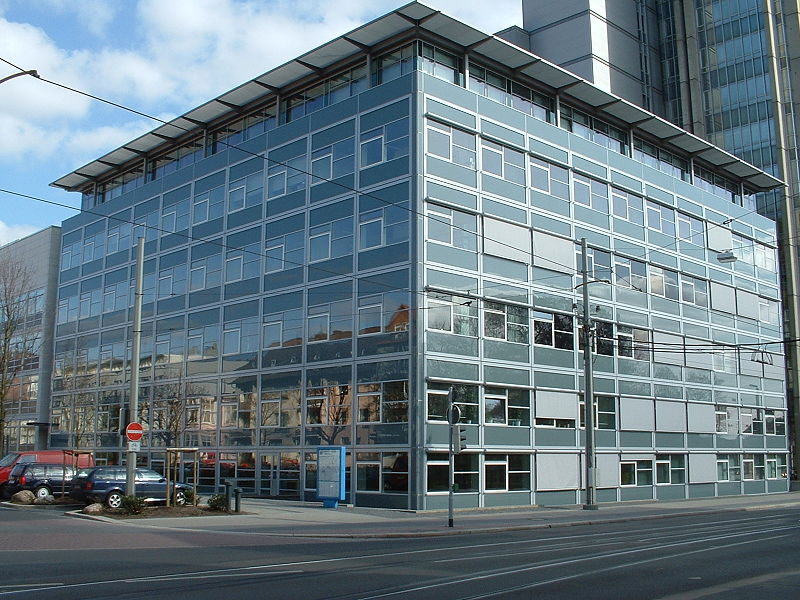
\includegraphics{infozentrum.jpg}}
%\titlegraphic[scaled]{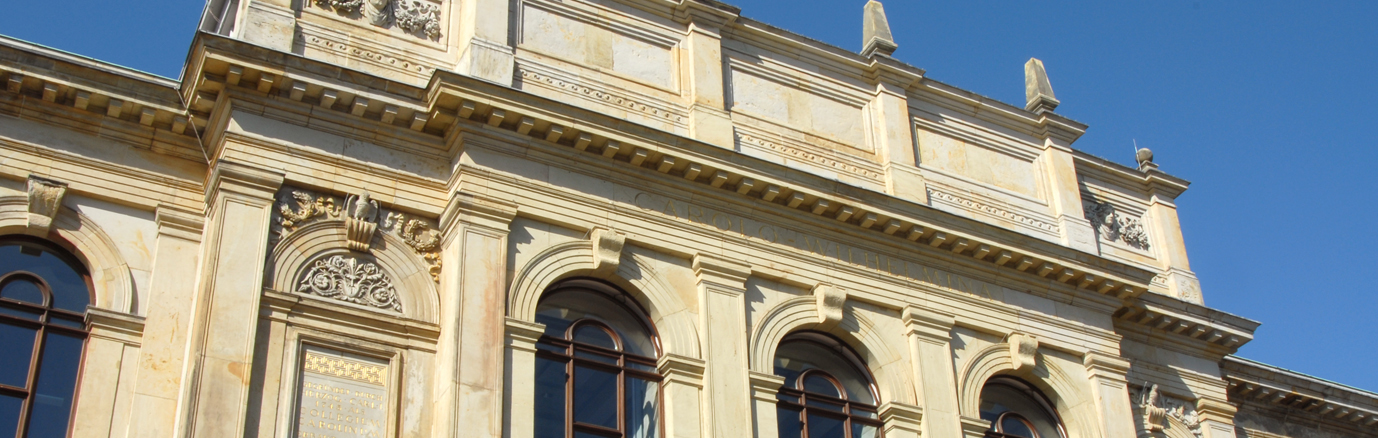
\includegraphics{titlepicture.jpg}}

% Logo, dass auf Titelseiten oben rechts und auf Inthaltsseiten unten rechts
% dargestellt wird. Es wird jeweils automatisch skliert
\logo{
\includegraphics{ibr_de_alternative.pdf}}
%\logo{Institut für Unkreativität\\und Schreibschwäche}

\usepackage{tikz}
\usetikzlibrary{arrows,automata,decorations.pathmorphing,backgrounds,shapes,positioning,fit,matrix,calc}
\usepackage{fourier-orns}

\newcommand{\catpic}[3][6cm]{
	\begin{tikzpicture}[remember picture,overlay]
	\begin{pgfonlayer}{background}
	\node[anchor=south east,outer sep=0pt,inner sep=0pt, align=left] (b) at ($(current page.south east) +(-0.05in,0.44in)$) {
		\parbox{#1}{
			\includegraphics[width=#1]{#2}\newline
			\centering \footnotesize #3
		}
	};
	\end{pgfonlayer}
	\end{tikzpicture}
}


%\newcommand{\good}{\Large\textcolor{tuGreenDark80}{\smiley{}}}
%\newcommand{\bad}{\Large\textcolor{red}{\danger}}

\usepackage{fontawesome}

\newcommand{\good}{\Large\textcolor{tuGreenDark80}{\faSmileO}}
\newcommand{\bad}{\Large\textcolor{red}{\faFrownO}}%\danger

\usepackage{calc}
\usepackage{printlen}
\newlength\imageheight
\newlength\imagewidth

\newlength\foo

\makeatletter
\newbox\@backgroundblock
\newenvironment{backgroundblock}[2]{%
	\global\setbox\@backgroundblock=\vbox\bgroup%
	\unvbox\@backgroundblock%
	\vbox to0pt\bgroup\vskip#2\hbox to0pt\bgroup\hskip#1\relax%
}{\egroup\egroup\egroup}
\addtobeamertemplate{background}{\box\@backgroundblock}{}
\makeatother

\newcommand{\pic}[3][6cm]{
	\parbox{#1}{
		\includegraphics[width=#1]{#2}\newline
		\centering \footnotesize #3
	}
}

\begin{document}

\begin{frame}[plain]
\titlepage
\end{frame}

\section*{Motivation}
%\begin{frame}{\insertsectionhead}
%	\begin{itemize}
%		\item[\good] Cloud-Computing fast überall
%		\item[\good] Outsourcing der Hardwarepflege 
%		\item[\good] Billige Rechenleistung
%		\item[\good] Leistung On-Demand
%	\end{itemize}
%	\catpic{Cloud_computing}{Cloud-Computing Übersicht \cite{CC}}
%\end{frame}

\begin{frame}{\insertsectionhead}
	\begin{itemize} % farben
		\item[\good] Cloud-Computing fast überall \vfill
		\item[\good] Auslagern der Hardwarepflege \vfill
		\item[\good] Billige Rechenleistung \vfill
		\item[\good] Leistung On-Demand \vfill
	\end{itemize}
\only<1>{
	%\begin{backgroundblock}{60mm}{30mm}
	%	\pic{Cloud_computing}{Cloud-Computing Übersicht \cite{CC}}
	%\end{backgroundblock}
	\catpic{Cloud_computing}{Cloud-Computing Übersicht \cite{CC}}
}
\only<2>{\catpic{Seal_of_the_United_States_National_Security_Agency}{NSA Logo \cite{NSA}}}
\pause
	\begin{itemize}
	\item[\bad] Daten werden manipuliert \vfill
	\item[\bad] Systemverhalten geändert \vfill
	\item[\bad] Anwendungen werden abgehört \vfill
\end{itemize}
\end{frame}

\begin{frame}{\insertsectionhead}
	Was wir wollen: \vfill
	\begin{itemize}
		\item Transparent für die Anwendung und das OS \vfill
		\item Anwendungen als Blackbox  \vfill
		\item Isolierte Anwendungen \vfill
		\item Keinem Vertrauen \vfill
	\end{itemize}
\vspace{1em}
	Was wir nicht beachten: \vfill
	\begin{itemize}
		\item Sicherheitslücken  \vfill
		\item Programmierfehler \vfill
		\item Side-Channel Attacken \vfill
		\item Denial-of-Service Attacken  \vfill
	\end{itemize}
	\catpic{into}{IBM Research Report \cite{boivie2013secureblue++:big}}
\end{frame}

\begin{frame}{Überblick}
	\tableofcontents
\end{frame}

\section{SecureBlue++~}
\begin{frame}{\insertsectionhead}
	\begin{itemize}
		\item Seit 2011 in Entwicklung \vfill
		\item Bisher keine reale Implementierung \vfill
		\item Sicheres, isoliertes Ausführen von Anwendungen \vfill
		\item Befehlssatzerweiterung für die POWER Architektur \vfill
		\begin{itemize}
			\item[$\Rightarrow$] Neue Register, Instruktionen \vfill
			%\item[$\Rightarrow$] Neue 
			\item[$\Rightarrow$] Geändertes Verhalten \vfill
			\item[$\Rightarrow$] Einzigartiger Schlüssel \vfill
			\item[$\Rightarrow$] Transparent für die Anwendung \vfill
			\item[$\Rightarrow$] Nahezu transparent für das OS \vfill
			%\item[$\Rightarrow$] Interne Verwaltungsdatenstrukturen
		\end{itemize}
	\end{itemize}
\catpic{ibm}{IBM Logo \cite{ibm}}
	%\catpic[5cm]{ram}{Grundidee \cite{boivie2013secureblue++:big}}
\end{frame}

\subsection{Funktionsweise}

\begin{frame}{\insertsectionhead -- Neue Register und ROMs}
	\begin{itemize}
		\item Secure Executable ID Save/Restore \vfill
		\begin{itemize}
			\item \emph{SEIDSR} \vfill
		\end{itemize}
		\item Secure Executable ID \vfill
		\begin{itemize}
			\item \emph{SEID} \vfill
		\end{itemize}
		\item Eigener Private/Public Key \vfill
	\end{itemize}
	\catpic[5cm]{hw_key2}{Schlüssel \cite{boivie2013secureblue++:big}}
\end{frame}

\begin{frame}{\insertsectionhead -- Interne Datenstrukturen}
	\begin{itemize}
		\item Secure Executable Table (\emph{SET}) -- global \vfill
		\begin{itemize}
			\item \emph{SEID} \vfill
			\item Hash-Wert der Metadaten (\emph{MRMT}, Zeiger auf \emph{TRL}, Signal Handler \ldots)  \vfill% unterpunkt und beide Punkte zusammen fügen
			\item Zeiger auf Metadaten  \vfill
		\end{itemize}
		\item Memory Region Mapping Table (\emph{MRMT}) -- lokal \vfill
		\begin{itemize}
			\item AES-Schlüssel \vfill
			\item Große und Start der Region im Speicher \vfill
		\end{itemize}
		\item Protected Memory Table (\emph{PMT}) -- global \vfill
		\begin{itemize}
			\item \emph{MRID} \vfill
			\item \emph{SEID} des Erstellers \vfill
			\item Größe und Start der Region im Speicher \vfill
			\item AES-Schlüssel \vfill
		\end{itemize}
		\item Thread Restore List (\emph{TRL}) -- lokal \vfill
		
	\end{itemize}
	%\catpic{ibm}{IBM Logo \cite{ibm}}
\end{frame}

\begin{frame}{\insertsectionhead -- Verhalten}
	\begin{itemize}
		\item RAM-Verschlüsselung  \vfill
		\begin{itemize}
			\item Anwendungseigener AES-Schlüssel \vfill
		\end{itemize} \vspace{1em}
		\item Cache-Line-Schutz und Validierung \vfill
		\begin{itemize}
			\item Integrity Tree Validierung \vfill
			\item \emph{MRID} Labeling  \vfill
		\end{itemize}  \vspace{1em}
		\item Register-Schutz \vfill
		\begin{itemize}
			\item Bei jedem Interrupt \vfill
			\item CPU sichert Register in \emph{TRL} \vfill
			\item Nur \texttt{SEID}-Register bleibt \vfill
			\item Nicht bei \texttt{sesc}-Instruktion \vfill
		\end{itemize}
	\end{itemize}
%	Metadaten je gesicherter Anwendung: % weg
%\begin{itemize}
%	\item Signal Handler
%	\item \emph{MRMT}
%	\item Zeiger auf die \emph{TRL}
%\end{itemize}
	\catpic[5.8cm]{ram}{Grundidee \cite{boivie2013secureblue++:big}}
\end{frame}

\begin{frame}{\insertsectionhead -- Integrity Tree}
	\begin{itemize}
		\item Menge von Hash-Werten des Speichers %\vfill
		\item Knoten werden durch Elternknoten geschützt %\vfill
		\item Dient zum Schutz des Speichers vor Manipulationen %\vfill
		\item Initiale Zustand wird \texttt{esm} in Metadata übergeben %\vfill
		%\item Erhöht die benötigten RAM-Zugriffe \vfill
	\end{itemize}
% bild von baum
	\catpic[4.5cm]{baum2}{Abstrakter Baum}
\end{frame}

\begin{frame}{\insertsectionhead -- Neue Instruktionen}
	\begin{itemize}
		\item \texttt{esm} \vfill
			\begin{itemize}
				\item Erstellt die Verwaltungsdaten \vfill
				\item Startet die Anwendung \vfill
				\item Privilegiert  \vfill
			\end{itemize}
		\item \texttt{restorecontext} \vfill
		\begin{itemize}
			\item Stellt die Register wieder her \vfill
			\item Privilegiert  \vfill
		\end{itemize}
		\item \texttt{deletecontext} \vfill
		\begin{itemize}
			\item Gibt die Ressourcen frei \vfill
			\item Privilegiert  \vfill
		\end{itemize}
		\item \texttt{sesc} \vfill
			\begin{itemize}
				\item Führt System Calls aus \vfill
			\end{itemize}
	\end{itemize}
	\catpic[6.5cm]{esm}{\texttt{esm}-Instruktion \cite{boivie2013secureblue++:big}}
\end{frame}

\subsection{System Calls}

\begin{frame}{\insertsectionhead -- System Calls}
	\vspace{-0.5em}
\begin{figure}
	\centering
	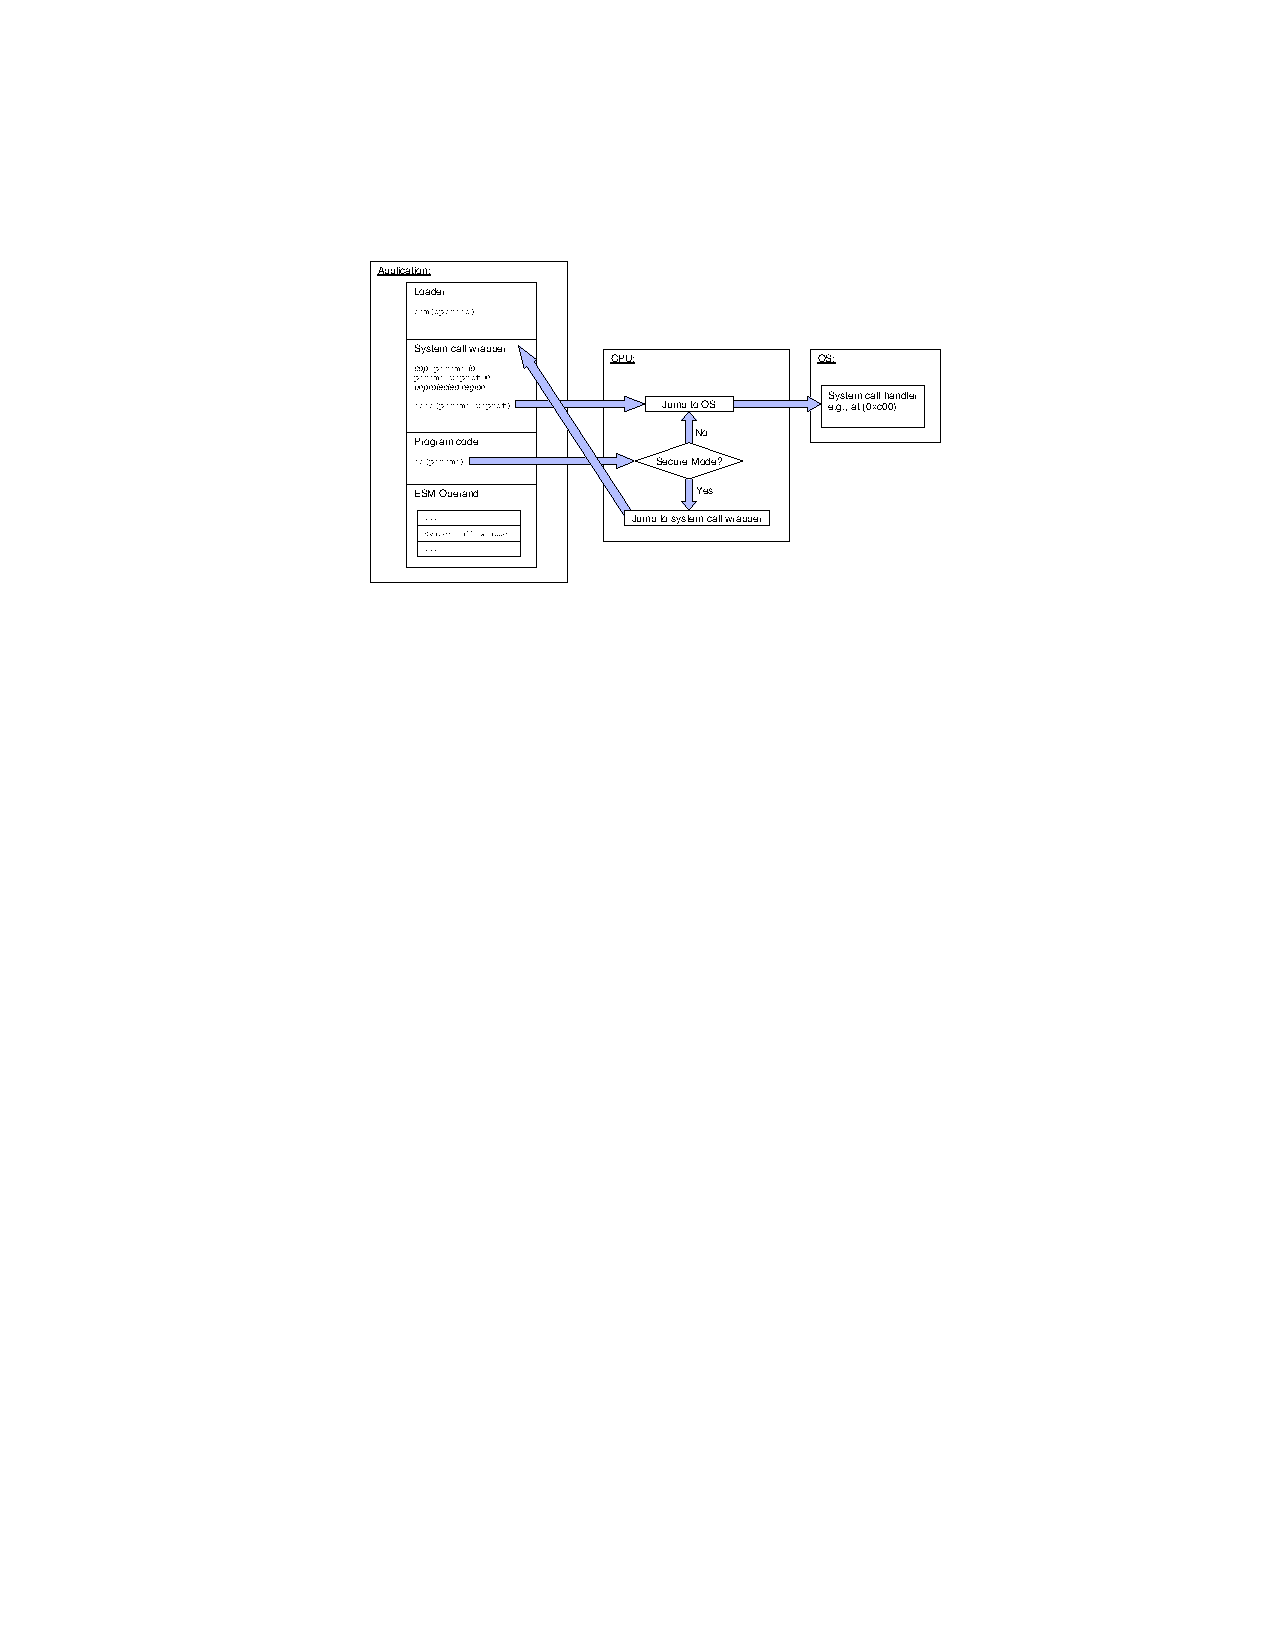
\includegraphics[width=\columnwidth]{sesc}
	\caption*{\footnotesize System Calls\cite{boivie2013secureblue++:big}}
	% nummerieren für die einzelnen schritte
\end{figure}
\end{frame}

\subsection{Anwendung}

\begin{frame}{\insertsectionhead -- Aufbau der ELF (Anwendung)}
	\begin{figure}
		\centering
		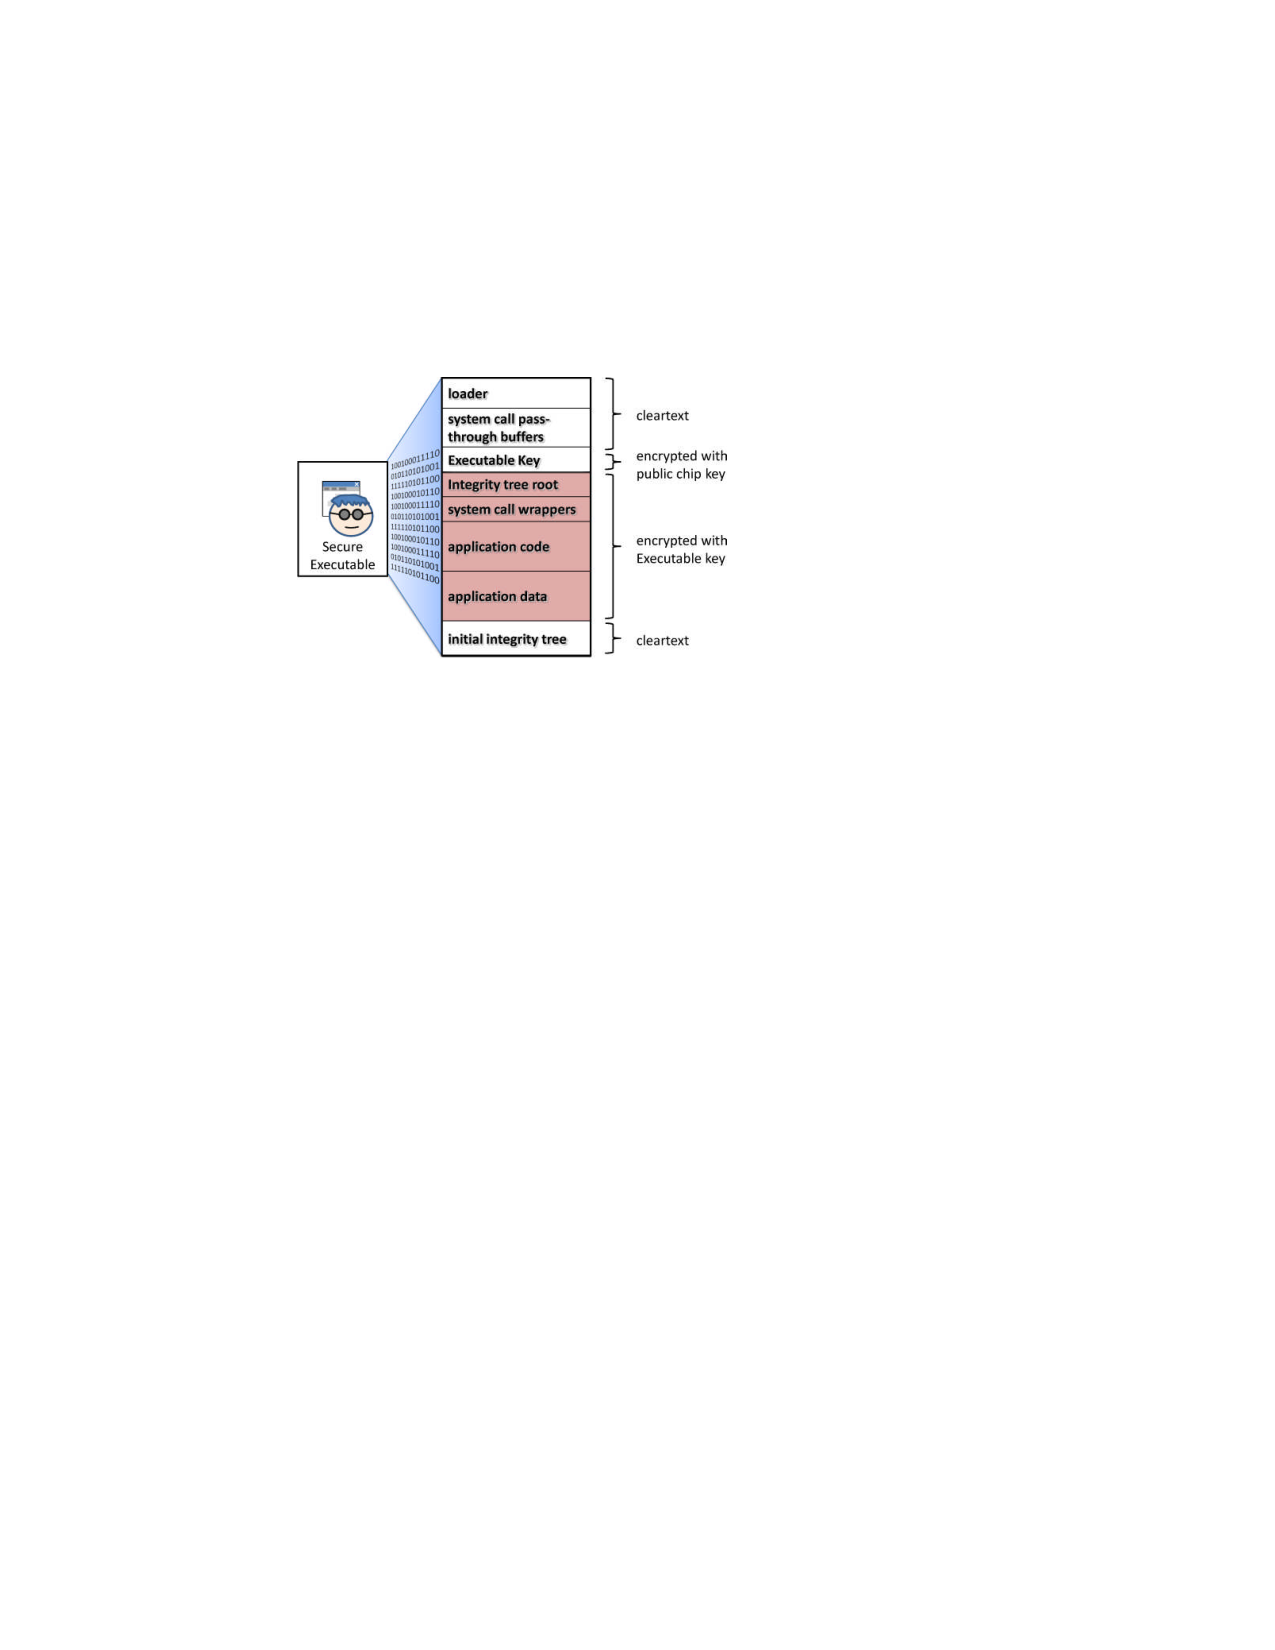
\includegraphics[width=.85\columnwidth]{aufbau}
		\caption*{\footnotesize Aufbau\cite{boivie2013secureblue++:big}}
	\end{figure}
% box vom schlüssel danbenen
\end{frame}

\subsection{Multithreading}

\begin{frame}{\insertsectionhead -- Multithreading}
	User Threads: \vfill
	\begin{itemize}
		\item Laufen auf Benutzerebene \vfill
		\item Eigener Scheduler im Programm ruft \texttt{restorecontext} auf \vfill
	\end{itemize} \vspace{1em}
	Kernel Threads: \vfill
	\begin{itemize}
		\item Kernel Verwaltet die Threads \vfill
		\item Viele Zustände für eine Anwendung \vfill
		\begin{itemize}
			\item Einen pro Thread \vfill
			\item Gespeichert in \emph{TRL} \vfill
		\end{itemize}
	\end{itemize}
\end{frame}

\subsection{Virtuelle Maschinen}

\begin{frame}{\insertsectionhead -- Virtuelle Maschinen}
	\begin{columns}
		\column{.6\textwidth}
		Hardware VM: \vfill
		\begin{itemize}
			\item Bevorzugt, weniger Leistungseinbußen % bei High-performance \vfill
			\item Gleiches Verhalten wie ohne VM  \vfill % anderes Wort \vfill
			\item Domain $0$ ruft \texttt{restorecontext} auf \vfill
		\end{itemize} \vspace{1em}
		Software VM: \vfill
		\begin{itemize}
			\item Benötigt Anpassungen \vfill
			\item Gast OS als sichere Anwendung \vfill
			\item Anwendung als virtuelle sichere Anwendung \vfill
		\end{itemize}
		\column{.3\textwidth}
			\vspace{-.5em}
			\begin{figure}
			\centering
			\begin{subfigure}[b]{\columnwidth}
				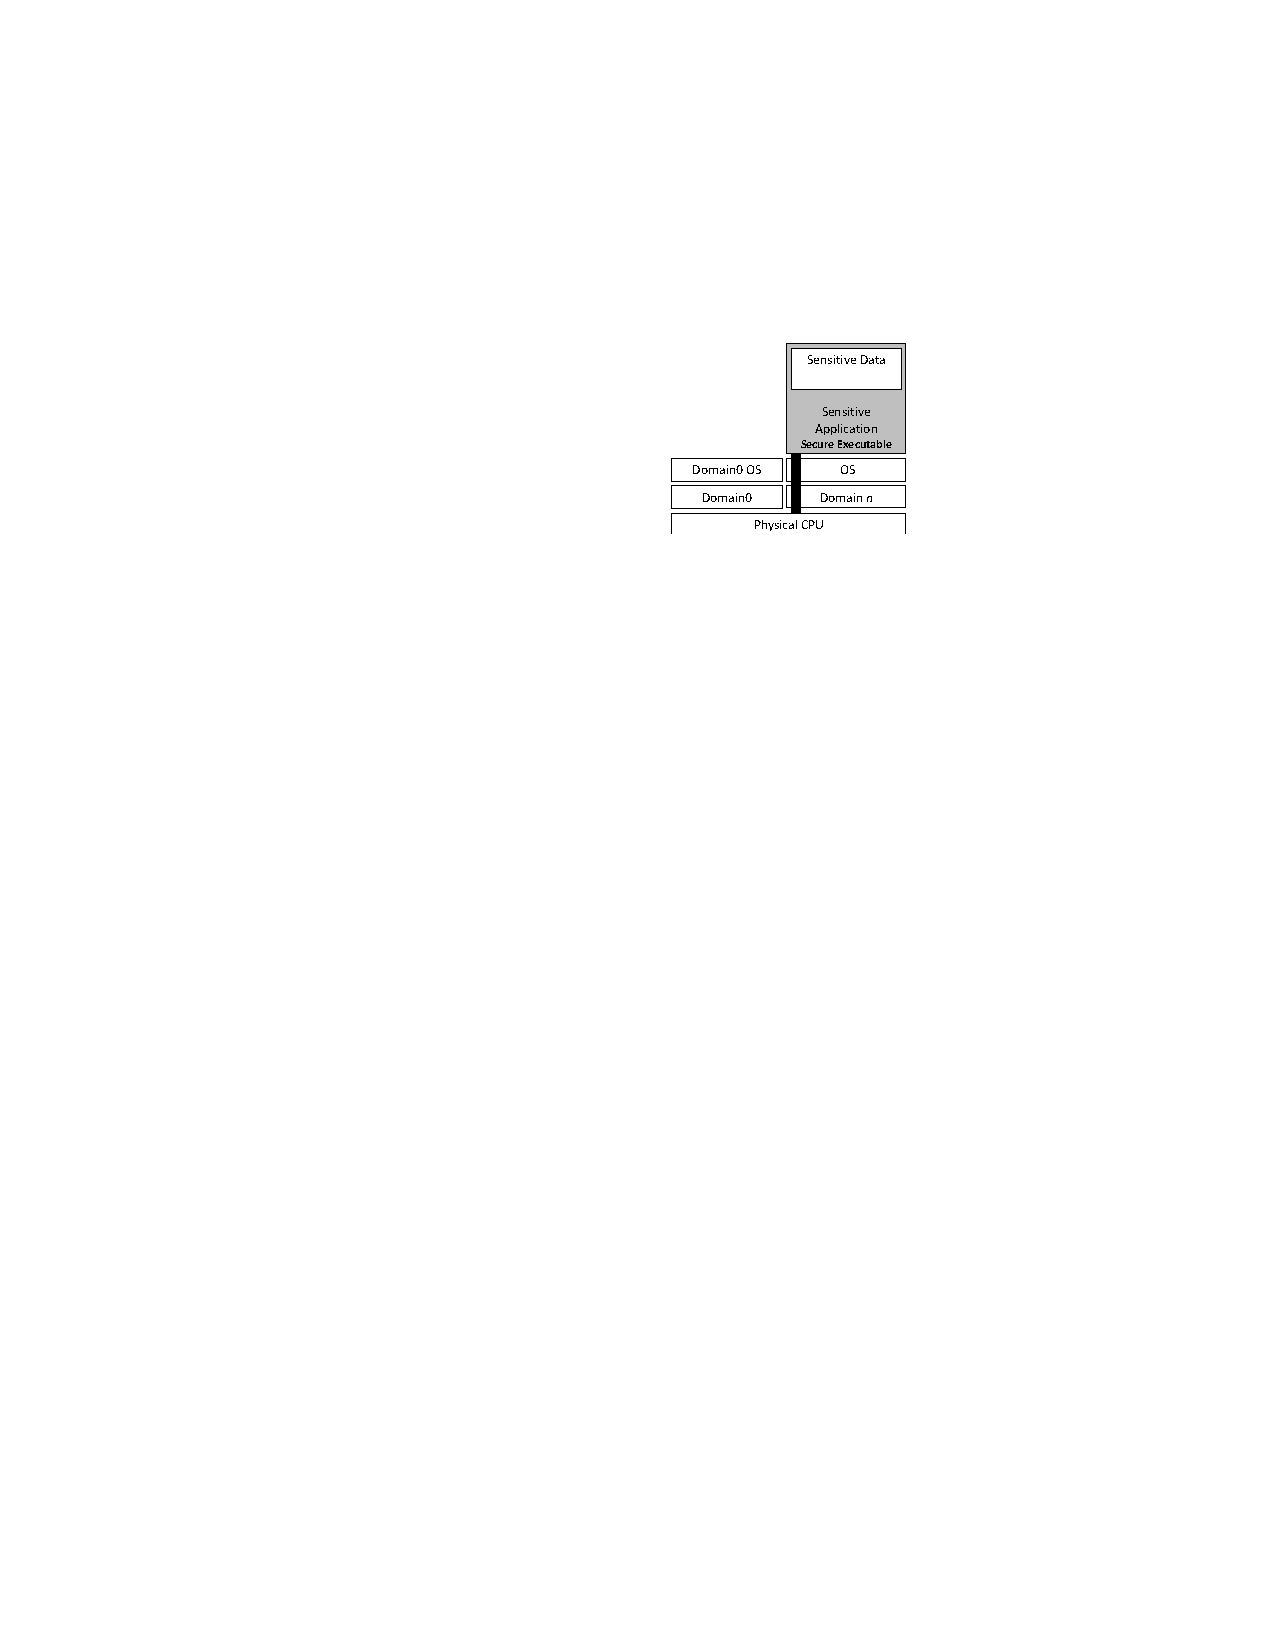
\includegraphics[width=.8\columnwidth]{hvm2}
				\caption*{\footnotesize Hardware VM\cite{boivie2013secureblue++:big}}
				\label{fig:hvm}
			\end{subfigure}
			\\
			\begin{subfigure}[b]{\columnwidth}
				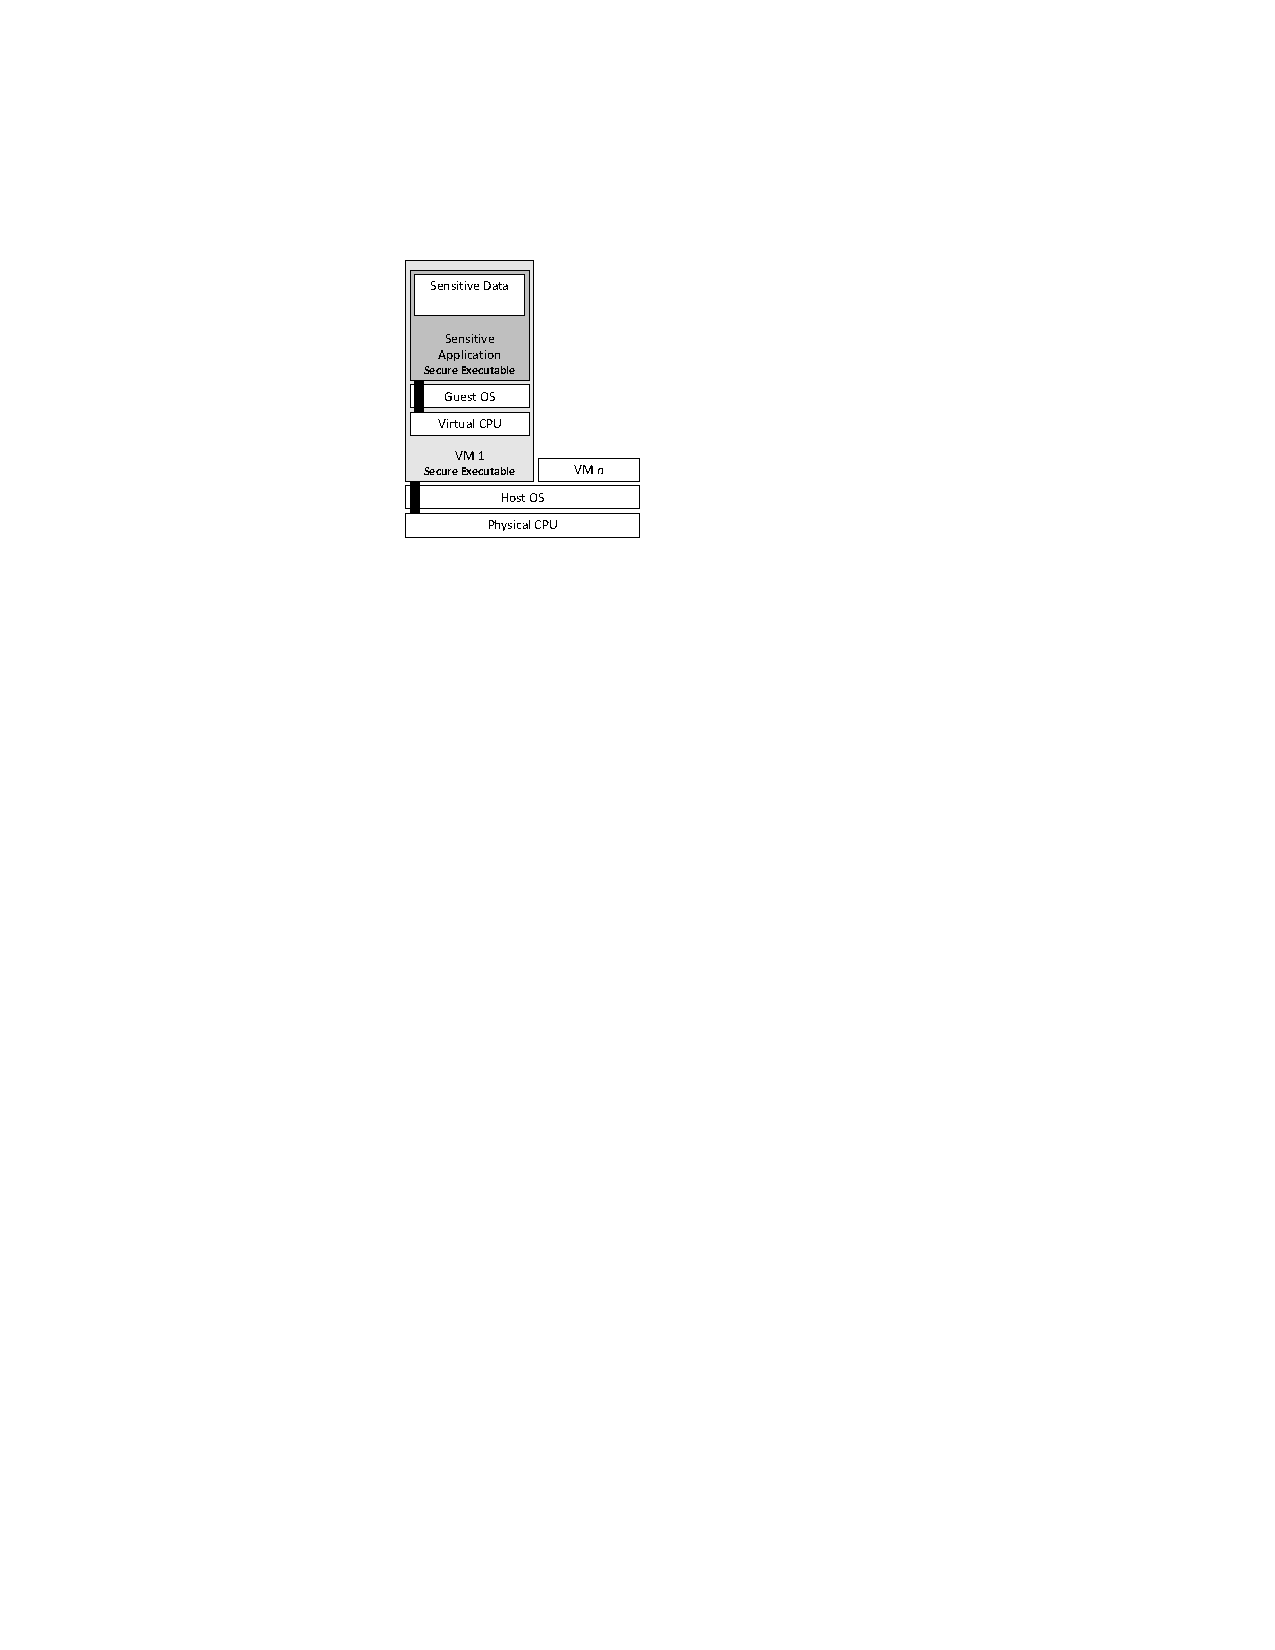
\includegraphics[width=.8\columnwidth]{svm}
				\caption*{\footnotesize Software VM\cite{boivie2013secureblue++:big}}
				\label{fig:svm}
			\end{subfigure}
			\label{fig:vms}
		\end{figure}
	\end{columns}
\end{frame}

\subsection{Benchmark}
\begin{frame}{\insertsectionhead -- Benchmark}
	\vspace*{-.7em}
	\begin{figure} % grün in andere Farbe ändern
		\centering
		\begin{subfigure}[b]{0.48\columnwidth}
			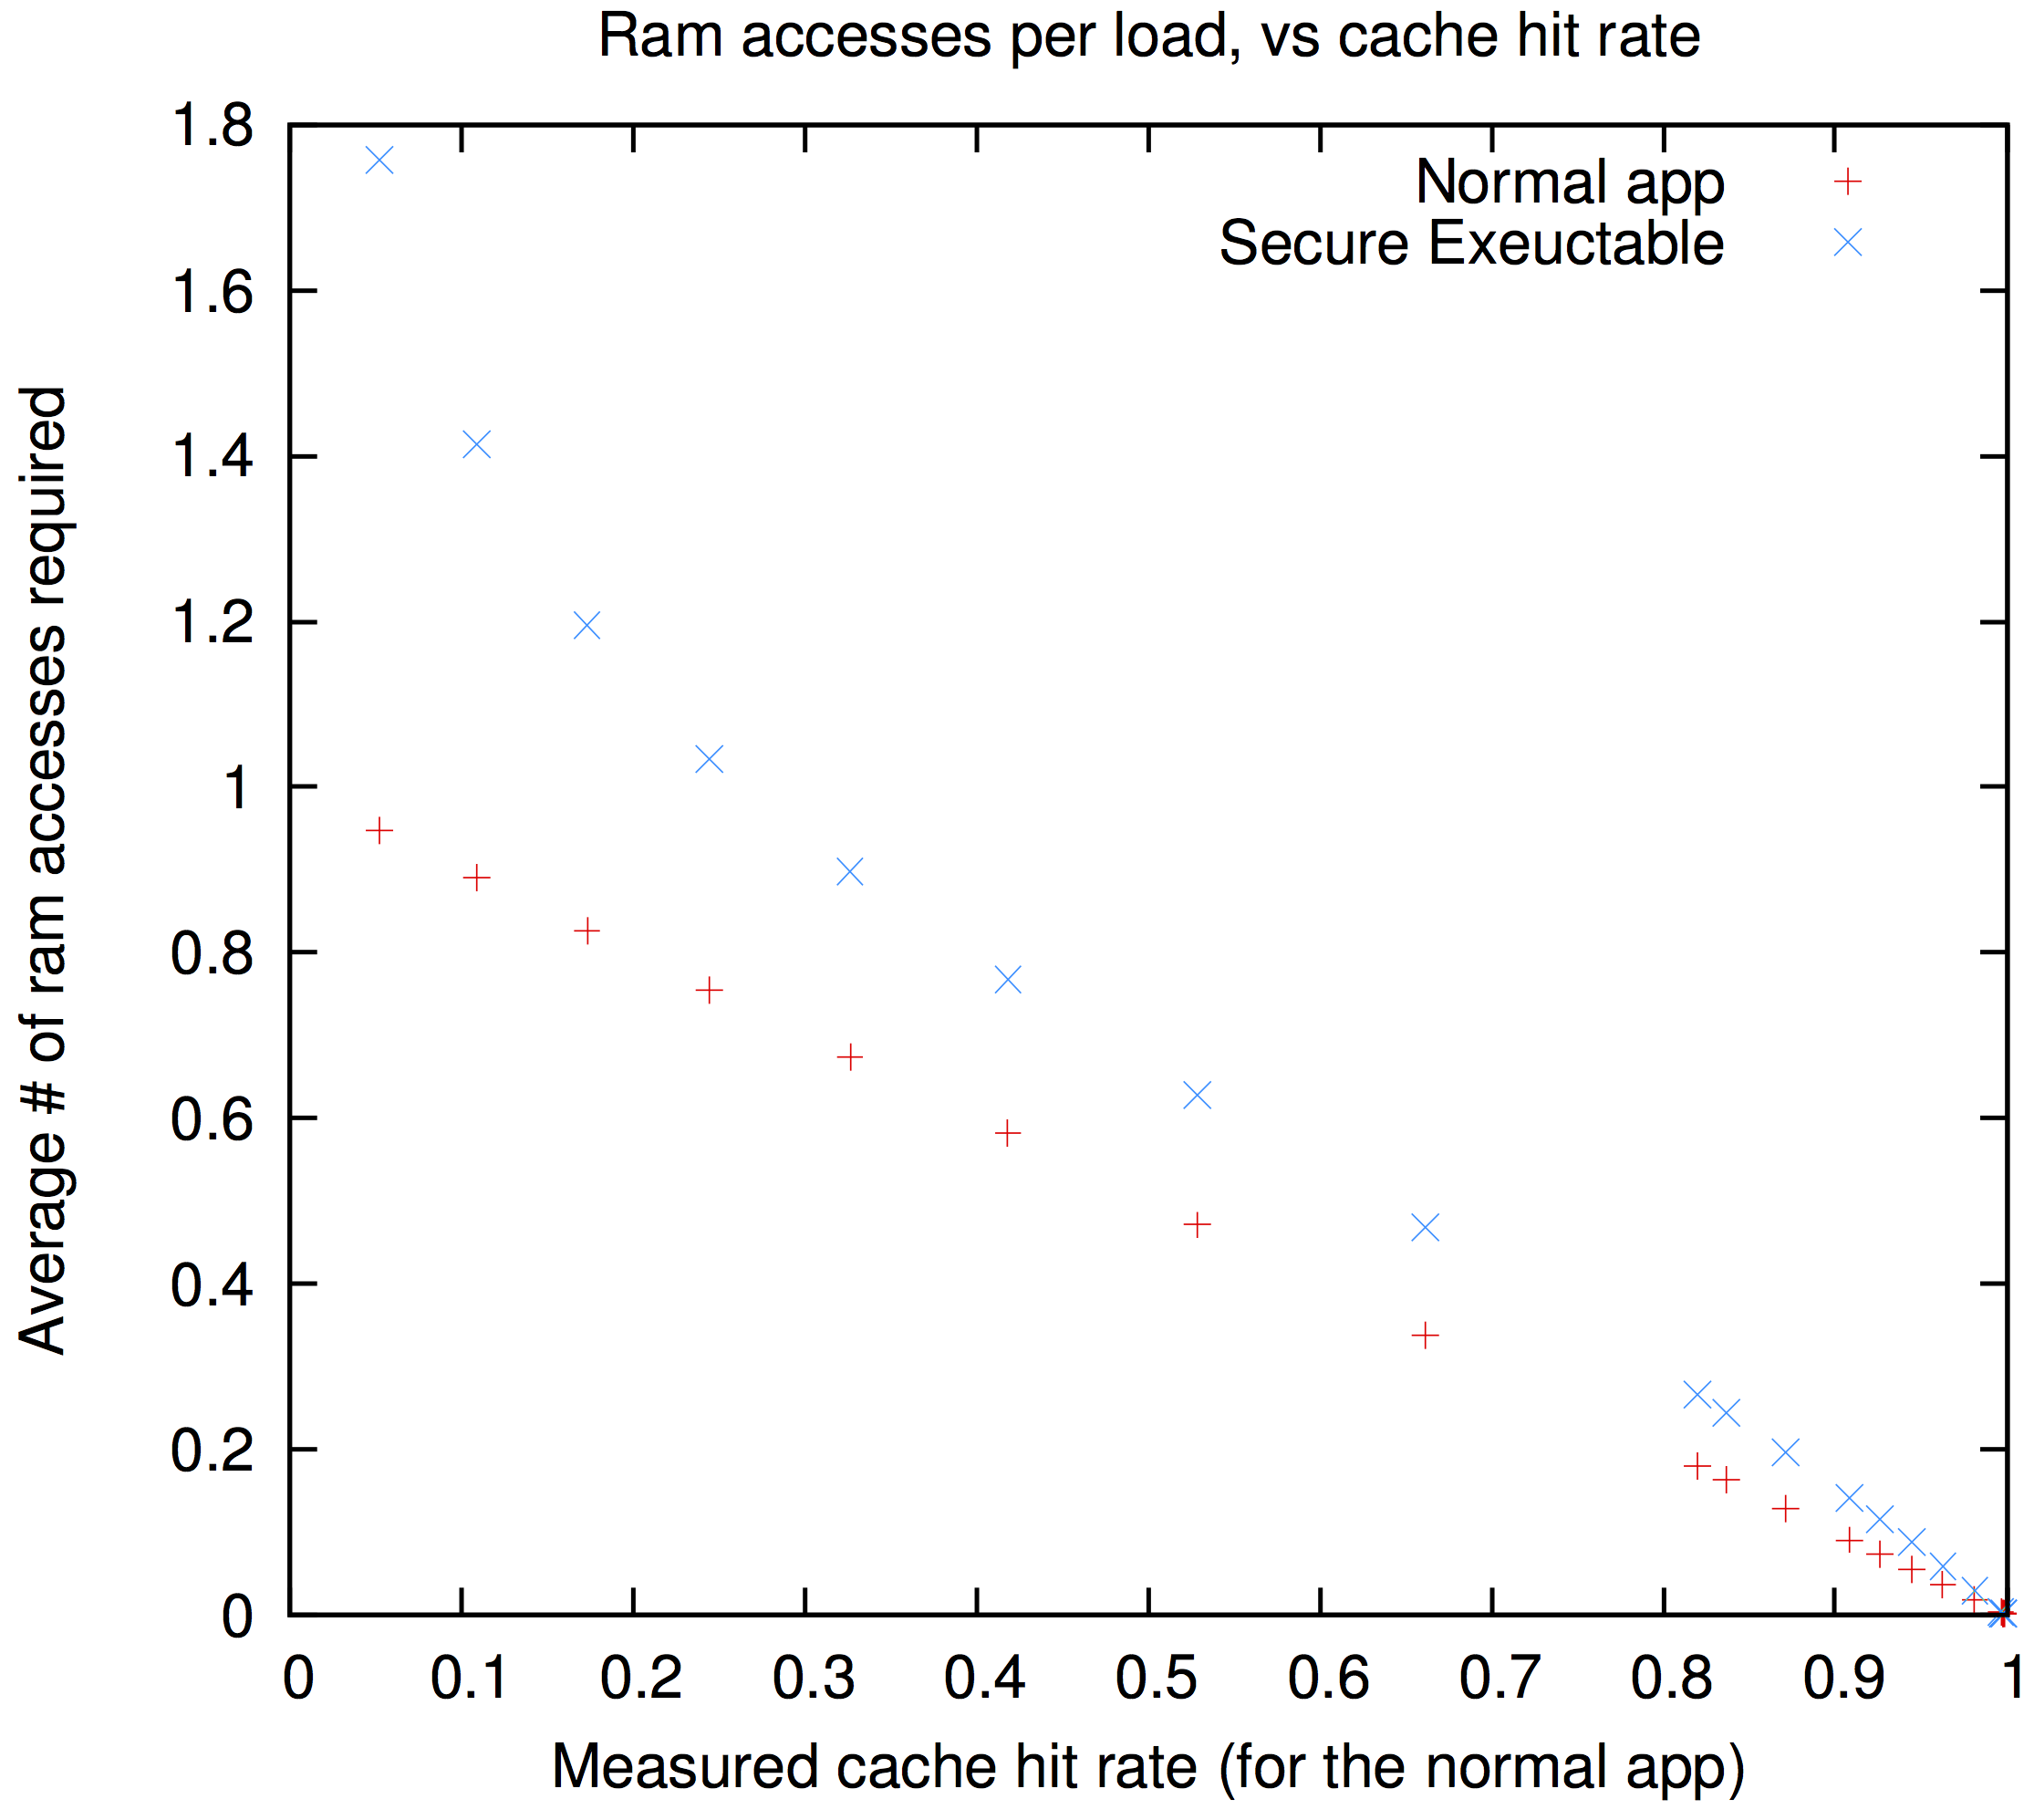
\includegraphics[width=\columnwidth]{bench_per_load2}
			\caption*{\footnotesize Lesen \cite{boivie2013secureblue++:big}}
			\label{fig:bench_load}
		\end{subfigure}
		\hfill
		\begin{subfigure}[b]{0.48\columnwidth}
			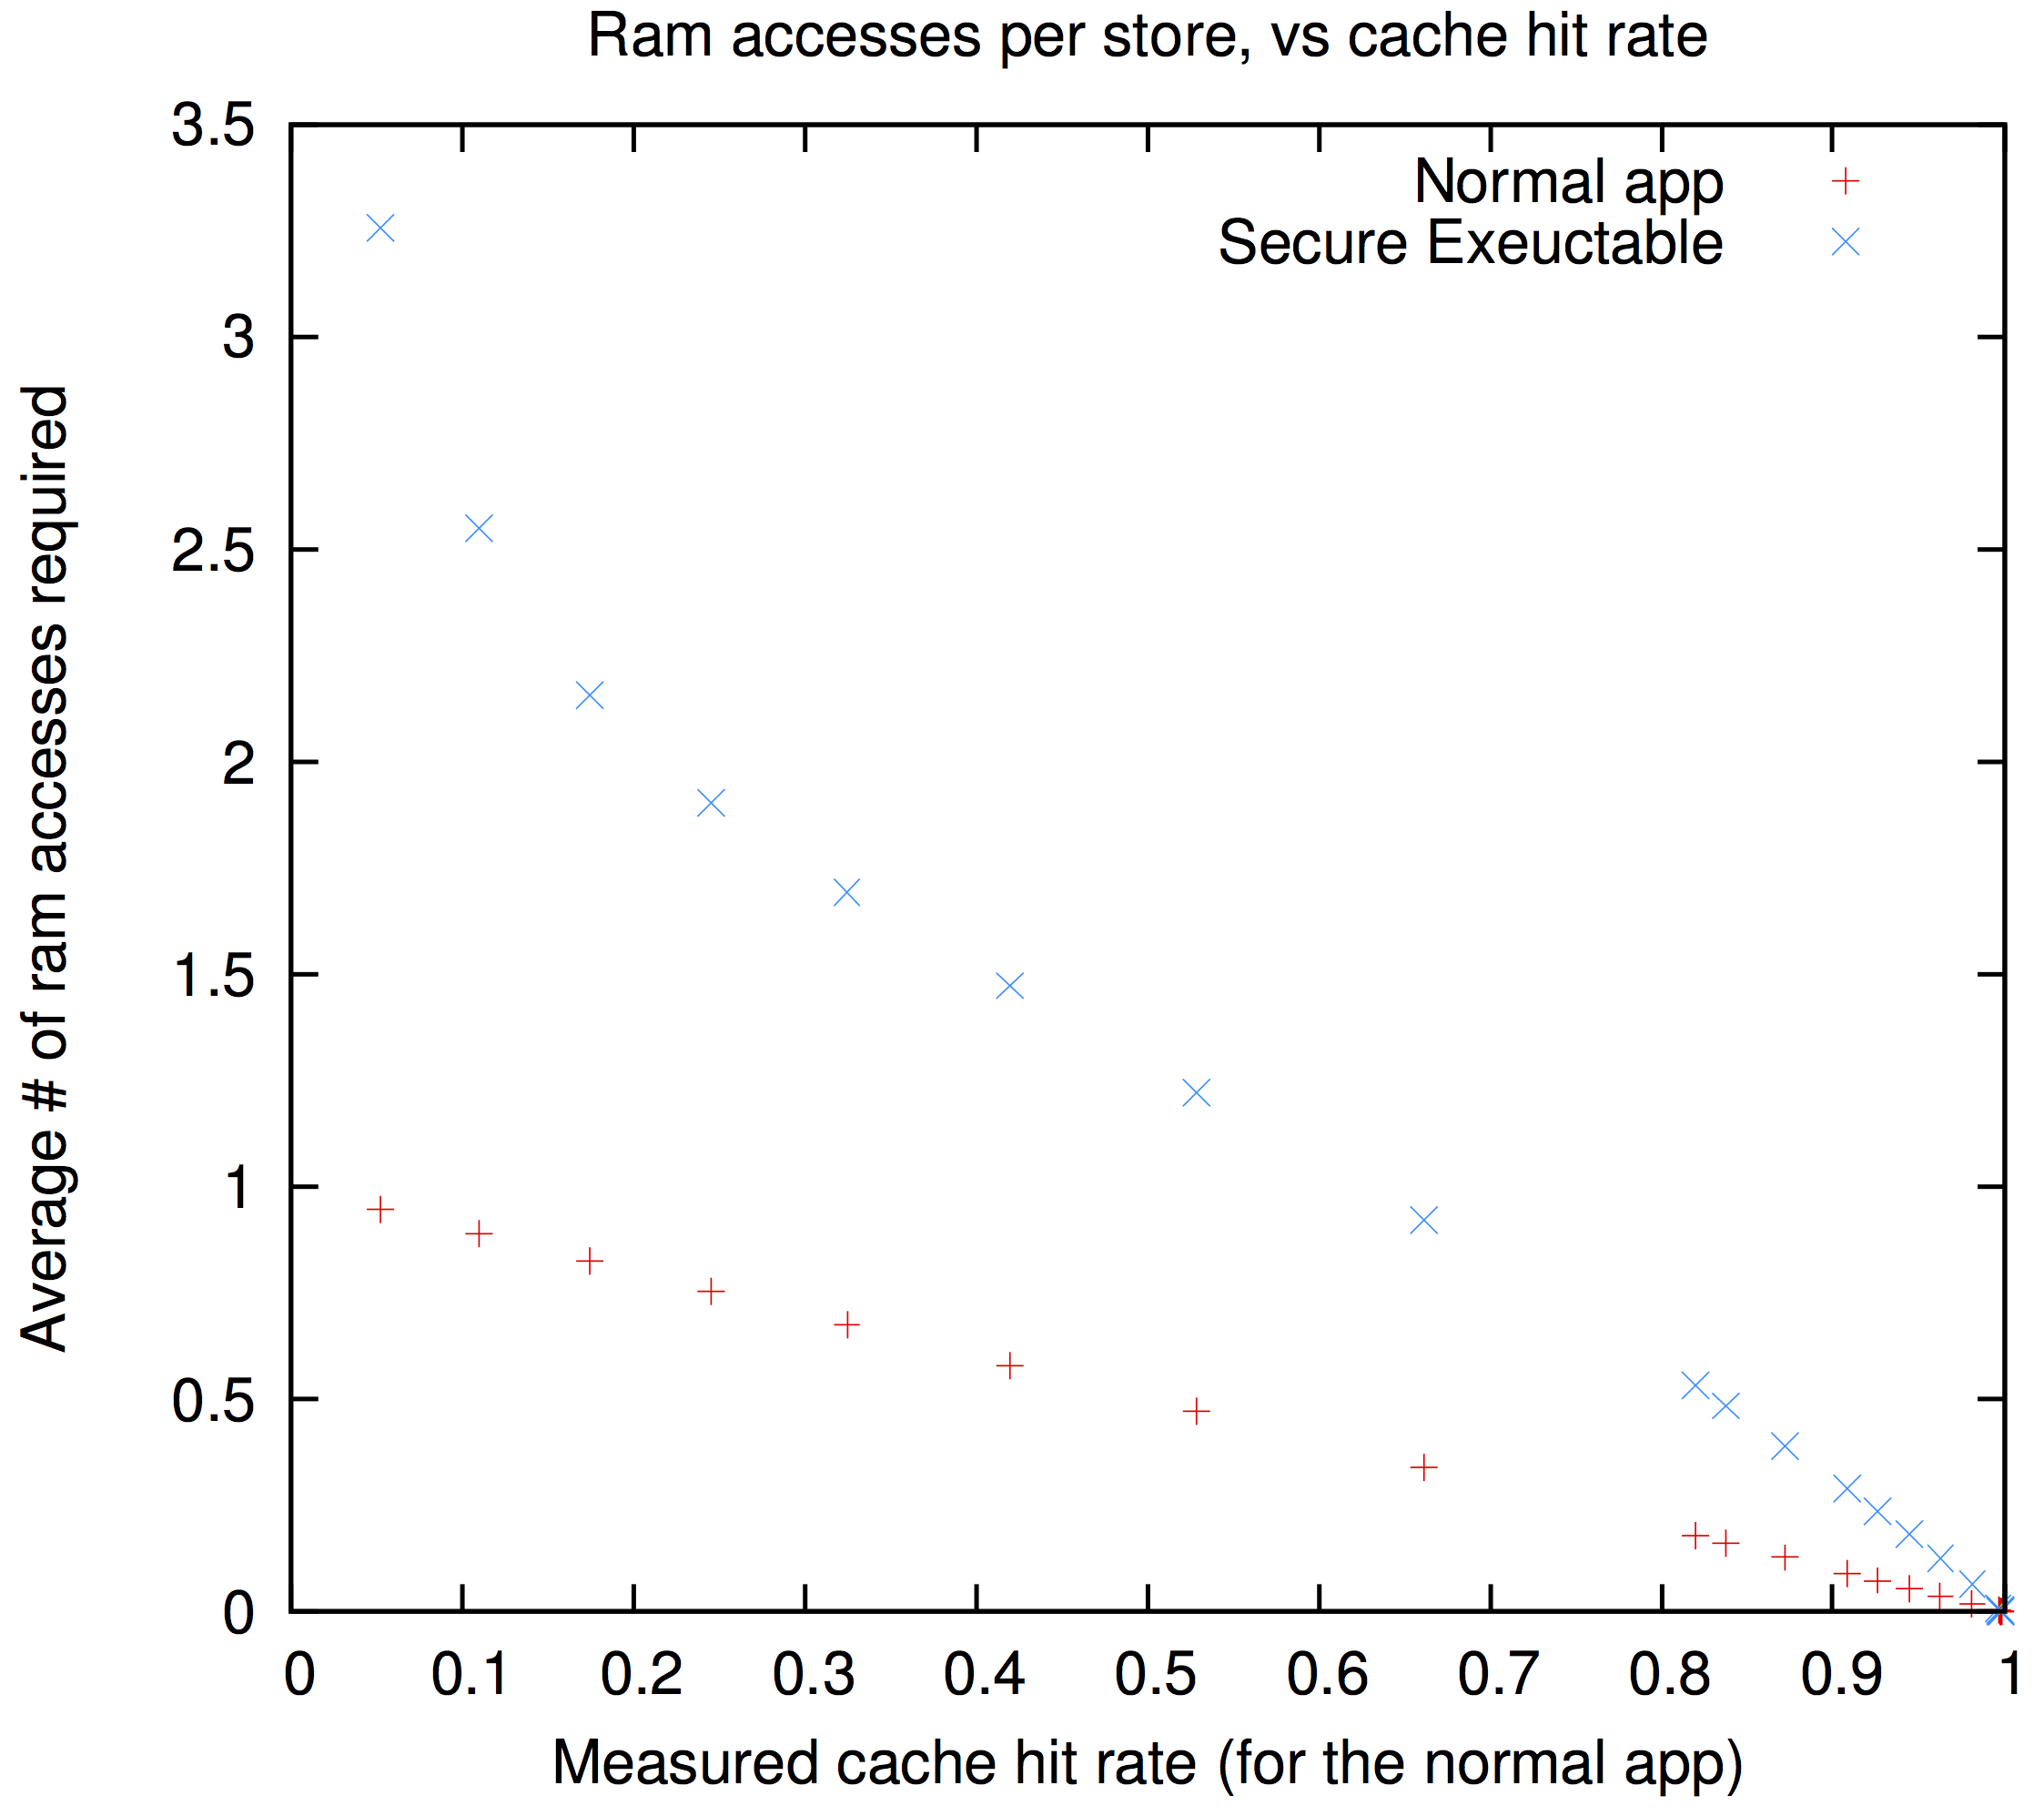
\includegraphics[width=\columnwidth]{bench_per_store2}
			\caption*{\footnotesize Schreiben \cite{boivie2013secureblue++:big}}
			\label{fig:bench_store}
		\end{subfigure}
		\label{fig:bench}
	\end{figure}
\vspace{-1.7em}
\begin{itemize}
	\item Sequenz von $10^6$ Adressen als Exponentialverteilung \vfill
	\item[\bad] Nur Simulation mit Cache Line-Validierung \vfill
	\item[\bad] Keine Verschlüsselung \vfill
\end{itemize}
\end{frame}

\section{Intel SGX~}
\begin{frame}{\insertsectionhead}
	\begin{itemize}
		\item Befehlssatzerweiterung von Intel \vfill
		\item Ermöglicht sichere und isolierte Ausführung \vfill
		\item In Skylake CPUs enthalten \vfill
		\item Limitiert auf 128MB RAM \vfill
		\end{itemize}
\catpic{intel2}{Intel Logo \cite{intel}}
\end{frame}

\subsection{Vergleich}
\begin{frame}{\insertsectionhead -- Vergleich}
	\begin{table}
		\centering
		\small
		\begin{tabular}{|p{5cm}|p{2.5cm}|p{2.5cm}|} \hline
			& SecureBlue++ & Intel SGX \cite{mckeen2013innovative} \\
			\hline 
			
			 Feinheit des Schutzes& \cellcolor{red!25}Prozess & \cellcolor{green!25}Virtuelle Speicherregion \\\hline
			 OS in der TCB& 	\cellcolor{green!25}N& 	\cellcolor{green!25}N \\\hline
			 Limitiert die Anwendung& 	\cellcolor{green!25}N& \cellcolor{green!25}N \\\hline
			 RAM Validierung hardwarebeschleunigt & \cellcolor{red!25}N& \cellcolor{green!25}J \\\hline
			 Dynamisch wachsender Speicher& \cellcolor{green!25}J & \cellcolor{red!25}N \\\hline
			 Anwendung ist Verschlüsselt& \cellcolor{yellow!25}J& \cellcolor{yellow!25}N \\\hline
			 Geheimnisse nur im speziellen Bereichen & \cellcolor{green!25}N  & \cellcolor{red!25}J\\\hline
			 Portabel & \cellcolor{red!25}N  & \cellcolor{green!25}J\\\hline
		\end{tabular}
		% Bindung der Anwendung
		%\caption*{Vergleich zwischen SecureBlue++ und SGX, Grün ist ein Vorteil und Rot eine Limitierung \cite{evtyushkin2014iso}}
		\caption*{\footnotesize Angelehnt an \cite{evtyushkin2014iso}}
	\end{table}
\end{frame}


\section{Zusammenfassung}
\begin{frame}{\insertsectionhead}
	\begin{itemize}
		% was wollten wir haben
		\item[\good] SecureBlue++ verspricht viel \vfill
		\item[\good] Isoliert Anwendungen \vfill
		\item[\good] Transparent für die Anwendung \vfill
		\item[\good] Geringe \emph{TBC} \vfill
		%\item OS muss \texttt{restorecontext}, \texttt{deletecontext} unterstützen
		% OS mus angepasst werden
		%\item Unbekannte Limitierung der \emph{SET}
		%\item Ungenaue Angaben zur \emph{MRMT} und \emph{PMT}
		% Implementierungsdetails sind ungenau
		\pause
		\item POWER Architektur \vfill
		\item Möglicherweise in den POWER9 CPUs enthalten \vfill
		\item[\bad] Bindung an eine CPU macht Cloud Computing nahezu unmöglich \vfill
		\item[\bad] Sehr wenig verfügbare ungenaue Informationen \vfill
		%\item Eignet sich als DRM-System
		\item[\bad] Lässt sich selbst für Malware missbrauchen \vfill
	\end{itemize}
\end{frame}

%\begin{frame}{Fragen?}
%\end{frame}

\begin{frame}{Danke}
	\centering
	Vielen Dank für die Aufmerksamkeit und das Interesse!
\end{frame}

\section*{Backup~}

\begin{frame}{\insertsectionhead -- System Calls}
	System Calls müssen selbst implementiert werden: \vfill
	\begin{itemize}
		\item \texttt{signal} \vfill
		\begin{itemize}
			\item OS kann nicht das \emph{PC}-Register ändern \vfill
			\item Eigener Signal Handler in den Metadaten \vfill
		\end{itemize}
		\item \texttt{fork} \vfill
		\begin{itemize}
			\item Speicherbereich wird kopiert \vfill
			\item Eigentümer in \emph{SET} wird geändert \vfill
		\end{itemize}
		\item \texttt{clone} \vfill
		\begin{itemize}
			\item Eintrag in \emph{TRL}  \vfill
			\item Einträge dem Scheduler zur Verfügung gestellt  \vfill
		\end{itemize}
		\item \texttt{exit}  \vfill
		\begin{itemize}
			\item Programm wird in eine Endlosschleife versetzt \vfill
		\end{itemize}
	\end{itemize}
\end{frame}

\begin{frame}{\insertsectionhead -- Erstellen der Anwendung}
	\vspace{-0.3em}
	\begin{figure}
		\centering
		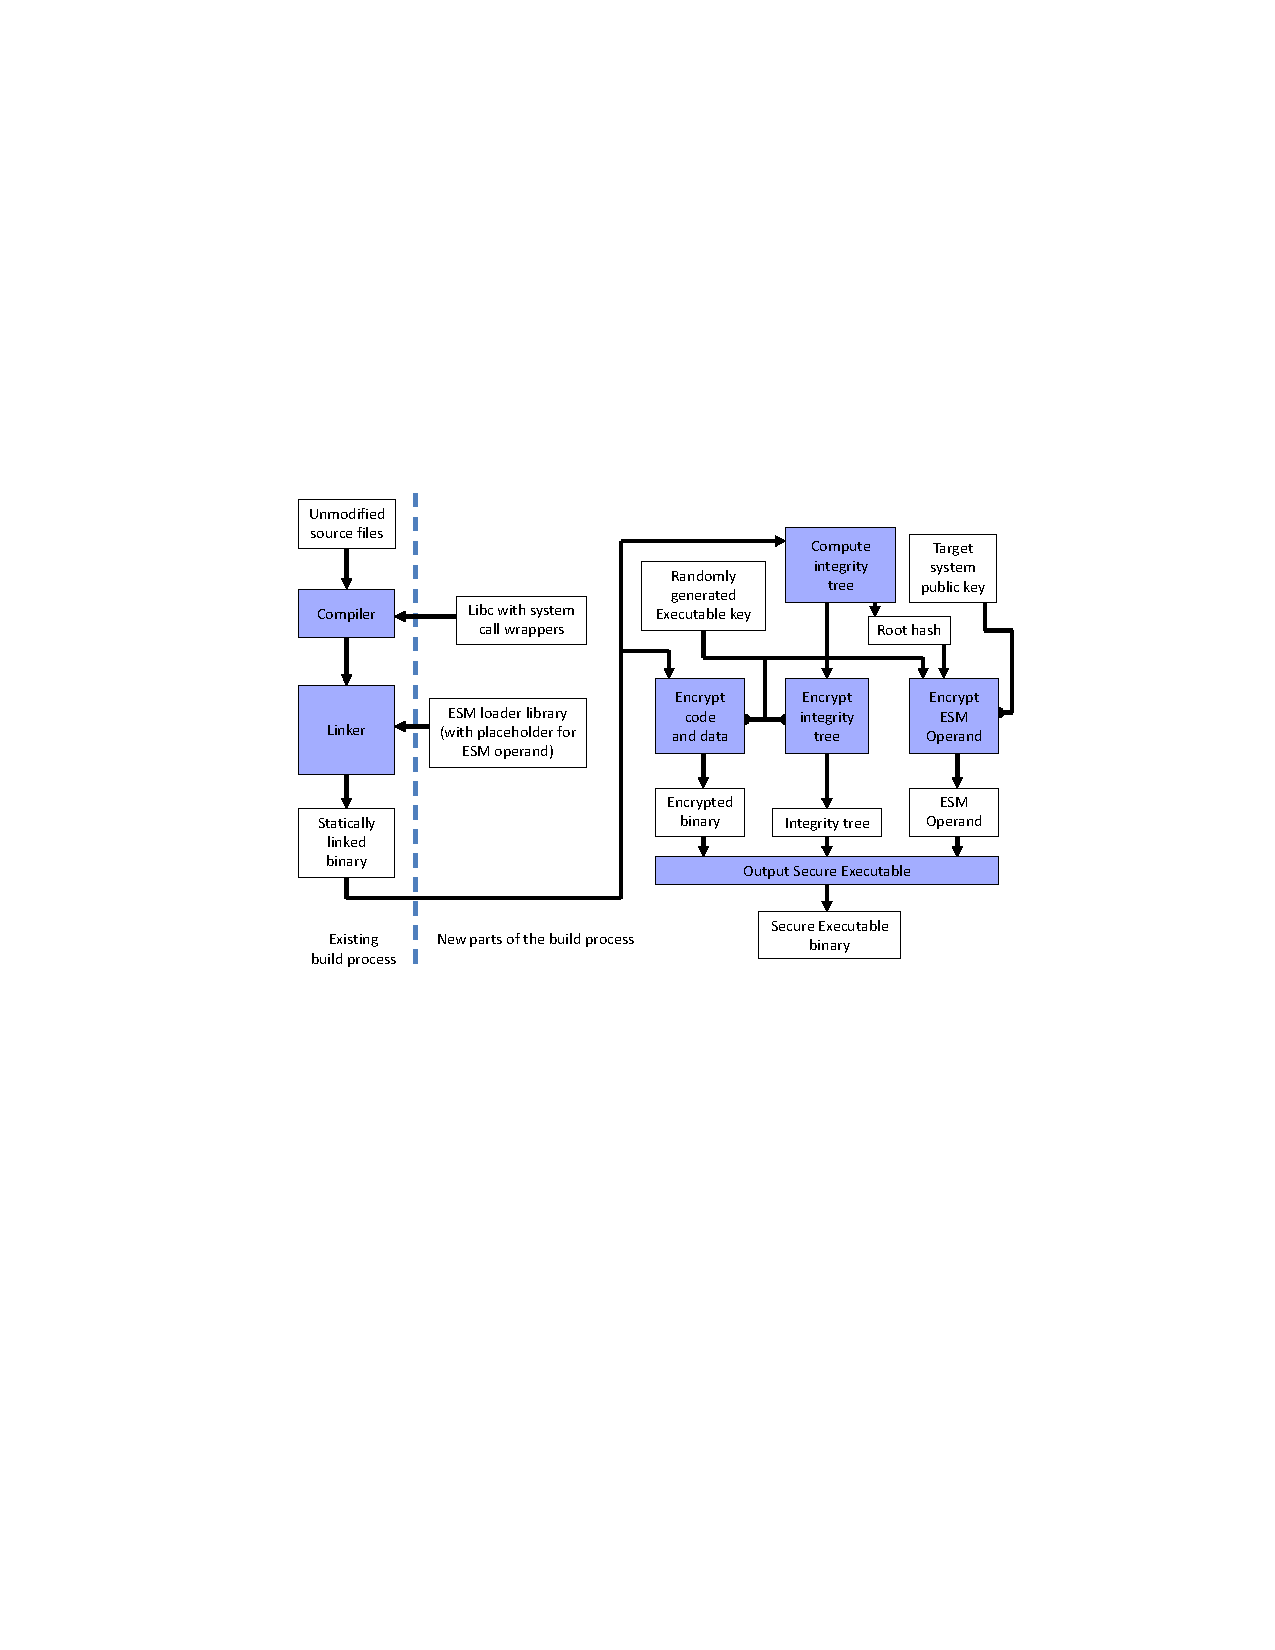
\includegraphics[width=.85\columnwidth]{build}
		\caption*{\footnotesize Erstellen\cite{boivie2013secureblue++:big}}
	\end{figure}
\end{frame}

\begin{frame}[allowframebreaks]{Quellen}
	\bibliographystyle{abbrv}	
	\bibliography{sigproc}  
\end{frame}

%
%\begin{frame}{\insertsectionhead}
%\end{frame}

\end{document}
